\documentclass[xcolor=pdftex,dvipsnames,table]{beamer}
\usetheme{Boadilla}
\usecolortheme{crane}
\usepackage[utf8]{inputenc}
\usepackage[english]{babel}
\usepackage{amsmath}
\usepackage{amscd}
\usepackage{amsfonts}
\usepackage{amssymb}
\usepackage{graphicx}
\usepackage{pgfplots}
\usepgfplotslibrary{fillbetween}
\usepackage{centernot}
\usepackage{mathrsfs} % x \mathscr fonts 
\usepackage{bm}
\usepackage{soul,xspace}
\usepackage{marvosym}
\usepackage{tikz}
\usetikzlibrary{positioning}
\usepgflibrary{shapes.arrows}
\usetikzlibrary{shapes.geometric,mindmap,fit}
\usepgflibrary{shapes.misc}
\usetikzlibrary{shadows}
\usetikzlibrary{arrows}
\usetikzlibrary{calc}
\let\labelstyle=\textstyle
\pgfdeclarelayer{background} \pgfdeclarelayer{foreground}
\pgfsetlayers{background,main,foreground}
%\usetikzlibrary{backgrounds}

\usepgflibrary{decorations.pathmorphing}
\usepgflibrary{decorations.text}

\usetikzlibrary{calc,shapes.geometric,shapes.symbols}
\usetikzlibrary{shapes.callouts}
\usetikzlibrary{patterns}

\def\G{\mathcal{\color{violet}G}}
\def\R{\mathbb{R}}
\def\bv{\mathbf{v}}
\def\bu{\mathbf{u}}
\def\res{\Rightarrow}
\def\AO{Agg}
\def\imp{\rightarrow}
\newcommand{\argmax}{\mathop{\mathrm{argmax}}}

\usepackage{listings}


\title{Learning and Reasoning in Logic Tensor Networks}
\subtitle{Hackaton Proposal} 
\author{Luciano Serafini\inst{1},
  Artur d'Avila Garces\inst{2},
  Dr Tillman Weyde\inst{2}}
\institute{
  \inst{1}Fondazione Bruno Kessler, Italy  \\
  \inst{2}City University London, UK }
\begin{document}

\begin{frame}
  \titlepage
\end{frame}

\begin{frame}
  \frametitle{Objective}
  \begin{itemize}
  \item LTN 101 
  \item Explain how it works on  a simple scenario; 
  \item Discusso some idea of further application (simple) scenario;
  \item Get more accountant with LTN;
  \item Start some development of the new scenario in LTN. 
  \end{itemize}
\end{frame}
\begin{frame}[fragile]
  \frametitle{LTN 101}
  \begin{itemize}
  \item install \texttt{python 2.7/3.5} or later;
  \item install \texttt{tensorflow} instructions at \url{https://www.tensorflow.org/install};
  \item get \texttt{logictensornetwork.py} and the code of the first
    example by cloning the git repository\scriptsize
    \begin{verbatim}
      git clone http://gitlab.fbk.eu/serafini/dagstuhl_hackaton_on_LTN.git
\end{verbatim}
  \end{itemize}
\end{frame}
\begin{frame}
  \frametitle{Simple example}
\begin{columns}
  \begin{column}[t]{0.5\textwidth}
    \begin{block}{Knowledge}
      $\small 
      \begin{array}{l}
        \color{red} domain = [0,1]^3 \\
        \color{blue}  A(a_1), A(a_2), A(a_3) \\
        \color{blue}  B(b_1), B(b_2), B(b_3) \\
        \color{blue}  A(c) \vee B(c) \\
        \color{blue} \forall x A(x)\rightarrow \neg B(x) \\
        \color{blue} \forall xy.(R(x,y) \rightarrow A(x)) \\
        \color{blue} \forall xy.(R(x,y) \rightarrow B(y)) \\
        \color{blue} R(a_1,d) \\
        \color{red}f(a_1)  = [1.0,0.0,0.0] \\
        \color{red}f(a_2)  = [0.7,0.0,0.2] \\
        \color{red}f(a_3)  = [0.9,0.2,0.1] \\
        \color{red}f(b_1) = [0.0,1.0,1.0] \\
        \color{red}f(b_2) = [0.1,0.8,0.7]\\
        \color{red}f(b_3) = [0.3,1.0,0.8] \\
        \color{blue}\forall x y ({\color{red} |f(y) - f(x)| <
        \frac{1}{2}} \rightarrow R(x,y))
      \end{array}
      $
    \end{block}
  \end{column}
    \begin{column}[t]{0.45\textwidth}
      \begin{alertblock}{\color{white}Queries}
        $
        \begin{array}{l}
          \color{blue} ? A(c) \\
          \color{blue}? B(c) \\
          \color{blue}? A(d) \\
          \color{blue}? B(d) \\
          \color{blue} ? A(x) | x \in [0,1]^3 \\
          \color{blue} ? B(x) | x \in [0,1]^3 \\
          \color{blue} ? R(x,y) | x,y \in [0,1]^3 \\
          \color{red}? f(c) \\
          \color{red}? f(d) \\
        \end{array}
        $
      \end{alertblock}
    \end{column}
  \end{columns}
\end{frame}  
\begin{frame}
  \frametitle{Simple example}
  \begin{center}
    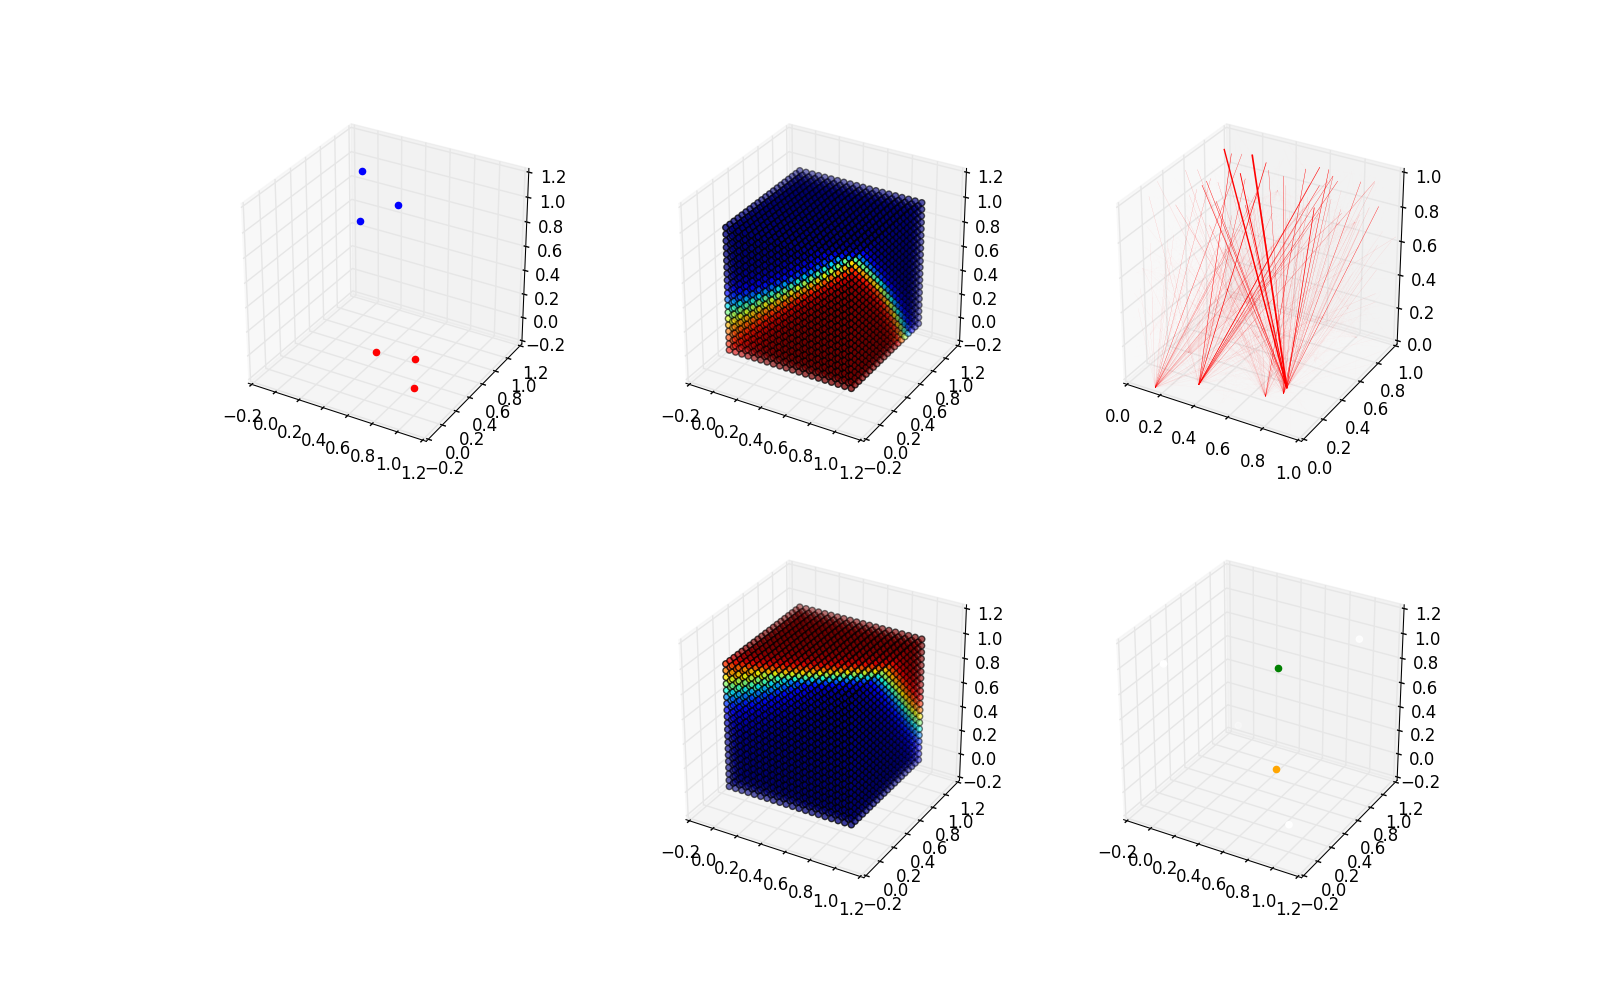
\includegraphics[width=\textwidth]{KebAB.png}
  \end{center}
\end{frame}
\begin{frame}
  \frametitle{\dots please join us .... it will be fun !!!!}
  \begin{center}
    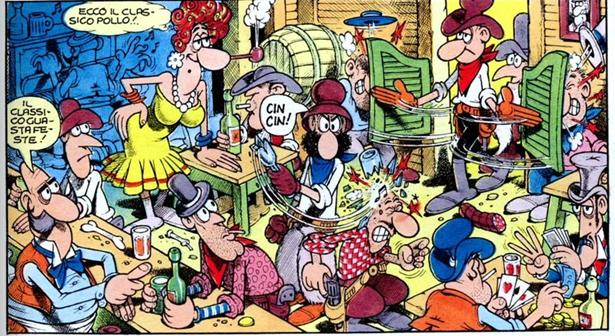
\includegraphics[width=\textwidth]{welcome.jpg}
  \end{center}
\end{frame}

\begin{frame}
  
\end{frame}
\end{document}
